\subsubsection{06.02.15}
\begin{enumerate}
	
	\item Время начала и окончания собрания: 20:00 - 21:00.
	
	\item Цели собрания: 
	\begin{enumerate}
		
		\item Ввести в функции управления ковшом промежуточное положение.
		
		\item Продолжить тренироваться.
		
	\end{enumerate}

	\item Проделанная работа:
	\begin{enumerate}
		
		\item Сегодня нами были приобретены игрушечные мячи, по размерам идентичные большим игровым мячам. Они значительно легче стандартных мячей, однако с ними тоже можно тренироваться.
		
		\item Мы подсчитали, что на заполнение подвижной корзины 90 см полностью требуется 13-14 мячей, поэтому мы решили тренироваться таким образом: выпустить на поле 3 оригинальных больших мяча и дополнить их еще 11 игрушечными, а также все маленькие мячи, что у нас есть (5 оригинальных и 18 мячей для настольного тенниса, соответствующих им по размеру), а затем наполнять корзину за минимальное время. Нам удалось заполнить корзину целиком за 2 минуты 40 секунд, что является неплохим результатом, но все же этого еще недостаточно для победы.
		\begin{figure}[H]
			\begin{minipage}[h]{0.2\linewidth}
				\center  
			\end{minipage}
			\begin{minipage}[h]{0.6\linewidth}
				\center{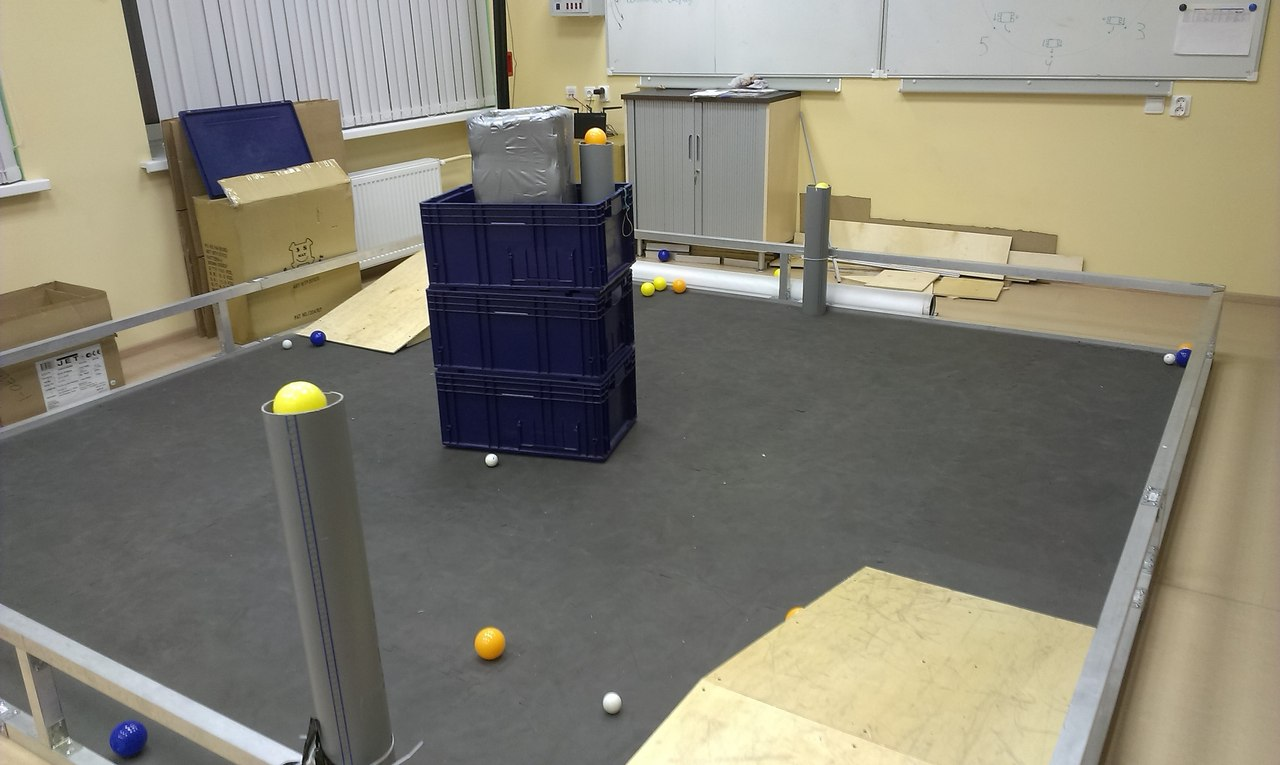
\includegraphics[scale=0.15]{days/06.02.15/images/01}}
				\caption{Наше игровое поле}
			\end{minipage}
		\end{figure}
		
        \item Программа управления ковшом была доработана и протестирована, результат положительный.
        \begin{figure}[H]
	  	  \begin{minipage}[h]{0.31\linewidth}
	  	    \center{
\includegraphics[scale=0.3]{days/06.02.15/images/03}}
	  	    \caption{Начальное положение}
	  	  \end{minipage}
	  	  \hfill
	  	  \begin{minipage}[h]{0.31\linewidth}
	  		\center{
\includegraphics[scale=0.3]{days/06.02.15/images/03}}
	  		\caption{Добавленное промежуточное положение}
	  	  \end{minipage}
	  	  \hfill
	  	  \begin{minipage}[h]{0.31\linewidth}
	  	   	\center{
\includegraphics[scale=0.3]{days/06.02.15/images/04}}
	  	   	\caption{Опрокинутый ковш}
	  	  \end{minipage}
	   \end{figure}

	\end{enumerate}
	
	\item Итоги собрания:
	\begin{enumerate}
		
		\item Мы успешно потренировались наполнять 90-сантиметровую подвижную корзину.
		
		\item Реализовано промежуточное положение ковша.
		
	\end{enumerate}
	
	\item Задачи для последующих собраний:
	\begin{enumerate}
		
		\item Продолжить тренировки.
		
		\item Реализовать программу автономного периода с пандуса.
		
		\item Реализовать защиту колес от наезда на мячи и палку-упор.
			
	\end{enumerate}
\end{enumerate}
\fillpage
